
%% The first command in your LaTeX source must be the \documentclass command.
\documentclass[acmsmall, nonacm, 11pt]{acmart}

\usepackage{subfig}
\graphicspath{{imgs/}}

\usepackage[ruled,vlined]{algorithm2e}
\usepackage{algorithmic}


%% The majority of ACM publications use numbered citations and
%% references.  The command \citestyle{authoryear} switches to the
%% "author year" style.
%%
%% If you are preparing content for an event
%% sponsored by ACM SIGGRAPH, you must use the "author year" style of
%% citations and references.
%% Uncommenting
%% the next command will enable that style.
%%\citestyle{acmauthoryear}

%%
%% end of the preamble, start of the body of the document source.
\begin{document}

%%
%% The "title" command has an optional parameter,
%% allowing the author to define a "short title" to be used in page headers.
\title{Project Report: Direct Visual Odometry for RGB-D Images}

%%
%% The "author" command and its associated commands are used to define
%% the authors and their affiliations.
%% Of note is the shared affiliation of the first two authors, and the
%% "authornote" and "authornotemark" commands
%% used to denote shared contribution to the research.
\author{Boqian Yu, 03708925}
\email{boqian.yu@tum.de}

%%
%% By default, the full list of authors will be used in the page
%% headers. Often, this list is too long, and will overlap
%% other information printed in the page headers. This command allows
%% the author to define a more concise list
%% of authors' names for this purpose.
\renewcommand{\shortauthors}{Boqian Yu}

%%
%% The abstract is a short summary of the work to be presented in the
%% article.
\begin{abstract}
  Due to its better usage of information provided in the input images, direct methods in the field of visual odometry have been receiving increasing focus in the past years. This report summarizes the practical project based on the robust direct visual odometry algorithm for RGB-D images, including its mathematical derivation and the manual implementation. Results based on the TUM-dataset are compared with those provided in the original paper to measure the performance of the implementation.
\end{abstract}

% Omit the "Author's Address" footnote
\makeatletter
\let\@authorsaddresses\@empty
\makeatother

%%
%% This command processes the author and affiliation and title
%% information and builds the first part of the formatted document.
\maketitle

\section{Introduction}
Simultaneous localization and mapping (SLAM) has wide applications in many fields, including autonomous driving\cite{levinson2011automatic}, geological survey \cite{kraus1998determination}, underground construction \cite{nuchter20046d} \cite{pejic2013design} etc. One of the most significant techniques of SLAM is the estimation and maintaining of the knowledge of robot poses and motions through real-time data typically either as point clouds (from laser scanners) or as image frames (from cameras), of which the latter is refered to as visual odometry and has been among the most popular topics in the past years.

Visual odometry algorithms can be categorized into two classes:
\begin{itemize}
    \item \textbf{Feature-based methods.} The idea of feature-based methods is to estimate the relative motion between two frames by only registering some feature observations extracted from the images. These features are usually computed using descriptors such as SIFT \cite{lowe1999object}, SURF \cite{bay2006surf}, ORB \cite{rublee2011orb}, BRIEF \cite{calonder2010brief} etc. with various criteria. However, feature-based methods discard information in the images that are not considered as "significant" by the chosen descriptor, although such information can also contribute to the motion estimation.
    \item \textbf{Direct methods.} Direct methods, on the other hand, overcome the disadvantage mentioned above by optimizing the motion estimation directly on the image intensities and thus enabling the use of all information contained in the images. In this way, higher accuracy can be achieved within less time (not necessary to select and match feature descriptors). The idea of direct methods for visual odometry have been widely expanded for different applications, such as in \cite{steinbrucker2011real}, \cite{stuhmer2010real}, \cite{newcombe2011dtam}, \cite{engel2014lsd}, \cite{engel2017direct} etc.
\end{itemize}

This report discusses the theory and implementation of the robust direct visual odometry algorithm proposed in \cite{kerl2013robust} and is formulated as follow: section 2 will discuss the detailed mathematical derivation of the algorithm, including the warping function, the optimization goal and methods and means to enhance robustness; section 3 will discuss the manual implementation that is completed in this project; section 4 will then show some results of this implementation based on the TUM-dataset and compare its performance with the reference results given in the original paper.

\section{Mathematical derivation}
The basic assumption of the robust DVO algorithm is that the same world point $\mathbf{p}$ observed in a successive pair of RGB-D frames $(\mathcal{I}_1, \mathcal{Z}_1)$ and $(\mathcal{I}_2, \mathcal{Z}_2)$ should yield identical intensity, i.e. 

\begin{equation*}
\mathcal{I}_{1}(\mathbf{x}) = \mathcal{I}_{2}(\tau(\boldsymbol{\xi}, \mathbf{x}))
\end{equation*}

\noindent where $\tau(\boldsymbol{\xi}, \mathbf{x})$ is the warping function that enables the pixel coordinate transformation between these two camera frames under a certain camera motion $\boldsymbol{\xi}$ ($\boldsymbol{\xi} \in \mathbb{R}^6$ in form of twist coordinates). The residual of a pixel $\mathbf{x}_i$ is defined as:

\begin{equation}
r_i(\boldsymbol{\xi}) := \mathcal{I}_2\left(\tau\left(\boldsymbol{\xi}, \mathbf{x}_i\right)\right)-\mathcal{I}_1\left(\mathbf{x}_i\right)
\label{residual}
\end{equation}

By computing the MAP estimation of the overall residuals and minimizing it w.r.t $\boldsymbol{\xi}$, the relative motion estimation problem is then transformed into a weighted least square problem and can be solved by standard methods.

Beyond this, a motion prior based on the camera motion of the previous pair and a weight function based on the observed distribution of residuals are introduced to enhance the robustness of the algorithm against noises and outliers; a image pyramid is also suggested in the paper to support the validity of local linearization in the optimization steps.

\subsection{Warping Function}

\begin{figure}[h]
    \centering
    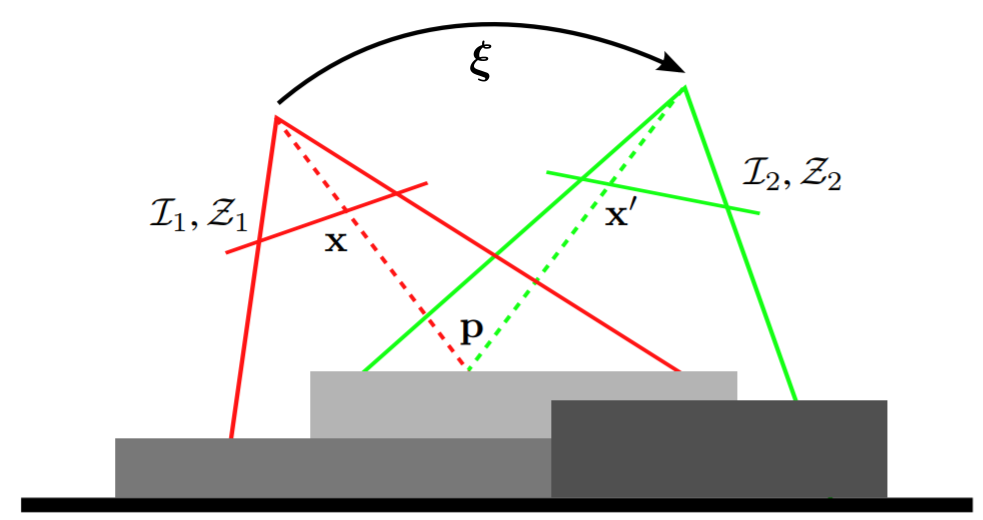
\includegraphics[width=0.6\linewidth]{imgs/warping.png}
    \caption{The warping function $\tau(\boldsymbol{\xi}, \mathbf{x})$ enables coordinate transformation $\mathbf{x}' = \tau(\boldsymbol{\xi}, \mathbf{x})$ between two frames under a certain relative motion $\boldsymbol{\xi}$ \cite{kerl2013robust}.}
    \label{warping}
\end{figure}

Consider a pinhole camera model with focal lengths $f_x, f_y$ and optical center $(c_x, c_y)$, the unprojection of a pixel $\mathbf{x} = (u, v)^{\top}$ in the frame of the first camera to its corresponding point $\mathbf{p}$ in the same frame can be written as:
\begin{equation}
\mathbf{p} = \pi^{-1}\left(\mathbf{x}, \mathcal{Z}_1(\mathbf{x})\right) = \mathcal{Z}_{1}(\mathbf{x})\left(\frac{u+c_x}{f_x}, \frac{v+c_y}{f_y}, 1\right)^{\top}
\label{unproject}
\end{equation}
\noindent where $\mathcal{Z}_1(\mathbf{x})$ refers to the depth value of this pixel in the first frame.

In order to transpose $\mathbf{p}$ into the frame of the second camera, a rigid body motion $g(\boldsymbol{\xi}) \in \mathrm{SE(3)}$ is applied to $\mathbf{p}$, which includes a rotation represented as a $3 \times 3$ orthogonal matrix $R \in \mathrm{SO(3)}$ and a translation represented as a $3 \times 1$ vector $\mathbf{t} \in \mathbb{R}^3$ and can be obtained from the twist $\boldsymbol{\xi}$ with $g(\boldsymbol{\xi}) = \mathrm{exp}(\hat{\boldsymbol{\xi}})$.

Apply the rigid body motion:
\begin{equation}
T(g(\boldsymbol{\xi}), \mathbf{p})=R \mathbf{p}+\mathbf{t}
\label{transform}
\end{equation}
and then project the transformed point $(X, Y, Z)^{\top} = T(g(\boldsymbol{\xi}), \mathbf{p})$ into the second frame:
\begin{equation}
\pi(T(g, \mathbf{p}))=\left(\frac{f_x X}{Z}-c_x, \frac{f_y Y}{Z}-c_y\right)^{\top}
\label{reproject}
\end{equation}

By summing up \eqref{unproject} \eqref{transform} \eqref{reproject}, the warping function between the two frames can be written as:

\begin{equation}
\tau(\boldsymbol{\xi}, \mathbf{x}) =\pi(T(g(\boldsymbol{\xi}), \mathbf{p})) = \pi\left(T\left(g(\boldsymbol{\xi}), \pi^{-1}\left(\mathbf{x}, \mathcal{Z}_1(\mathbf{x})\right)\right)\right)
\label{warpfunc}
\end{equation}

Although the procedures above are discussed merely with a pinhole camera model, they can actually be adapted to any camera model as long as the model complies with the intrinsic parameters specified by the dataset.

\subsection{MAP Estimation}

From the residual of each pixel defined in \eqref{residual}, a residual image between two frames can be formed by illustrating the residual of a pixel as brightness value, as shown in the example in Fig.  \ref{res_r}.

\begin{figure}[h]
    \centering
    \subfloat[\label{res_1}]{
        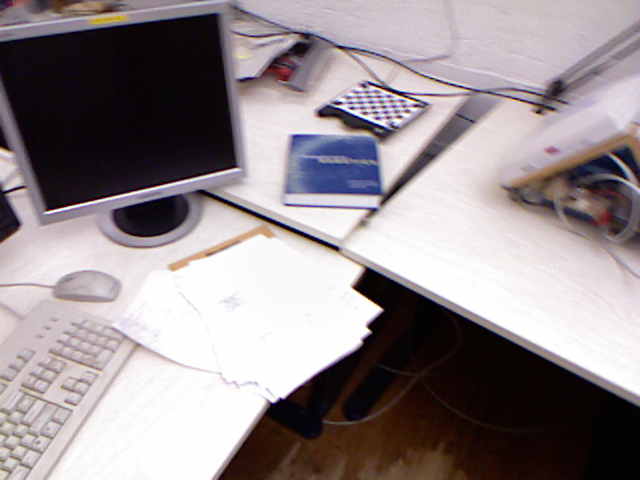
\includegraphics[width=0.3\linewidth]{res_1.png}}
    \subfloat[\label{res_2}]{
        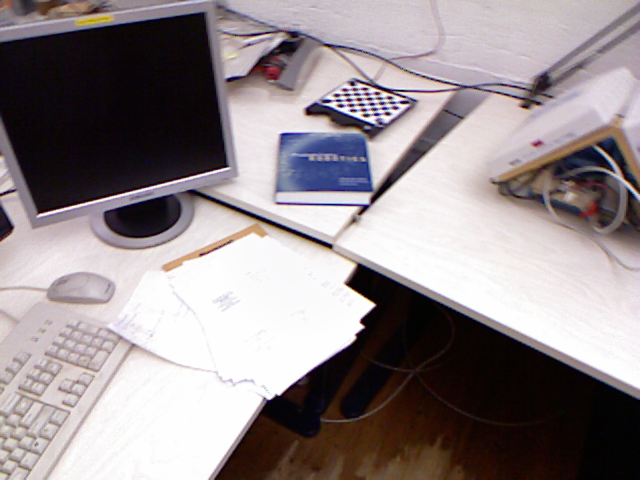
\includegraphics[width=0.3\linewidth]{res_2.png}}
    \subfloat[\label{res_r}]{
        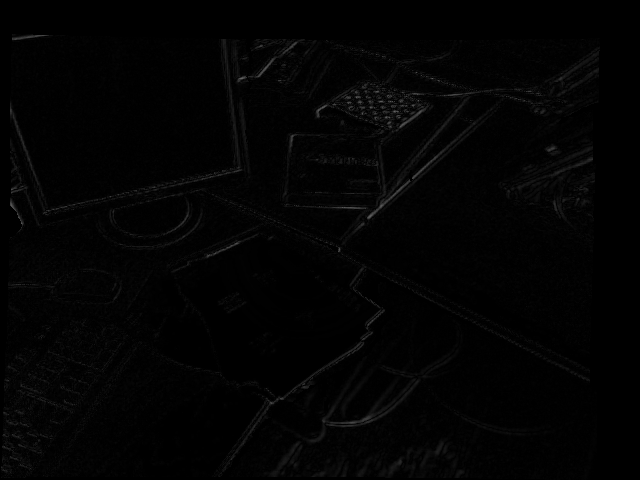
\includegraphics[width=0.3\linewidth]{res_r.png}}
    \caption{Two frames and the corresponding residual image. (a) RGB image of frame 1 (b) RGB image of frame 2 (c) residual image between the two frames}
    \label{img_residual}
\end{figure}

By assuming the independence and identical distribution of all pixels and stacking the residuals as $\mathbf{r} = (r_1, ..., r_n )^{\top}$, the overall likelihood can then be written as:
\begin{equation*}
p(\mathbf{r} | \boldsymbol{\xi})=\prod_{i} p\left(r_{i} | \boldsymbol{\xi}\right)
\end{equation*}
According to Bayes' law, the a posteriori likelihood of a relative camera motion $\boldsymbol{\xi}$ given the residual image can be formulated as:
\begin{equation}
p(\boldsymbol{\xi} | \mathbf{r})=\frac{p(\mathbf{r} | \boldsymbol{\xi}) p(\boldsymbol{\xi})}{p(\mathbf{r})}
\label{bayes}
\end{equation}
\noindent where $p(\boldsymbol{\xi})$ denotes the prior distribution over camera motion and $p(\mathbf{r})$ the distribution of residuals. These two parameters enable the integration of the prior knowledge of motion and residual distribution into the solution to achieve faster convergence and better robustness \cite{kerl2012odometry}, which will be discussed in later sections.

The item $p(\mathbf{r})$ can be neglected as it is not dependent on $\boldsymbol{\xi}$. The desired camera motion between the two frames can then be formulated as:

\begin{equation}
\begin{aligned}
\boldsymbol{\xi}_{\mathrm{MAP}} &= \arg \max _{\boldsymbol{\xi}} p(\mathbf{r} | \boldsymbol{\xi}) p(\boldsymbol{\xi}) \\
&=\arg \max _{\boldsymbol{\xi}} \prod_{i} p\left(r_{i} | \boldsymbol{\xi}\right) \cdot p(\boldsymbol{\xi}) \\
&=\arg \min _{\boldsymbol{\xi}} \sum_{i} -\log p\left(r_{i} | \boldsymbol{\xi}\right) - \log p(\boldsymbol{\xi})
\end{aligned}
\label{map_est}
\end{equation}

If the camera motion is assumed to be uniformly distributed, \eqref{map_est} can be further simplified as:

\begin{equation}
\boldsymbol{\xi}_{\mathrm{MAP}}=\underset{\boldsymbol{\xi}}{\arg \min } \sum_{i}^{n} -\log p\left(r_{i} | \boldsymbol{\xi}\right)
\label{sim_map}
\end{equation}

\noindent which can be solved by setting the derivative of the negative log-likelihood w.r.t. $\boldsymbol{\xi}$ to zero:

\begin{equation}
\sum_{i} \frac{\partial \log p\left(r_{i} | \boldsymbol{\xi}\right)}{\partial \boldsymbol{\xi}}=\sum_{i} \frac{\partial \log p\left(r_{i}\right)}{\partial r_{i}} \frac{\partial r_{i}}{\partial \boldsymbol{\xi}}=0
\label{deriv}
\end{equation}

By introducing a new symbol $w\left(r_{i}\right)=\frac{\log p\left(r_{i}\right)}{\partial r_{i}} \frac{1}{r_{i}}$, \eqref{sim_map} and \eqref{deriv} yields:

\begin{equation}
\boldsymbol{\xi}_{\mathrm{MAP}}=\underset{\boldsymbol{\xi}}{\arg \min } \sum_{i}^{n}\omega(r_i)(r_{i}(\boldsymbol{\xi}))^{2}
\label{rwls}
\end{equation}

\eqref{rwls} formulates the problem of solving the MAP estimation of the optimal camera motion for a pair of frames as a weighted least square problem, where $\omega(r_i)$ is the weighting function that decides how much a certain residual will contribute to the overall loss. Furthermore, if the residuals are normally distributed, i.e. $p\left(r_{i}\right)= \mathcal{N}\left(r_i, 0, \sigma^2\right)$, then all $\omega(r_i)$ are identical (and equal to $-1 /\sigma^2$), leading to a regular least square problem.

The above derivation assumes a uniform distribution for the camera motion, i.e. all possible sets of motion parameters are equally likely. By otherwise assuming a normal distribution for the camera motion, i.e. the motion prior $p(\boldsymbol{\xi})=\mathcal{N}\left(\boldsymbol{\xi}, \boldsymbol{\xi}_{0}, \Sigma_{\text {prior}}\right)$, a solution similar to \eqref{rwls} can be derived from \eqref{map_est}:

\begin{equation}
\boldsymbol{\xi}_{\mathrm{MAP}}=\underset{\boldsymbol{\xi}}{\arg \min } \sum_{i}^{n}\omega(r_i)(r_{i}(\boldsymbol{\xi}))^{2}+\Sigma_{\text{prior}}^{-1}\left(\boldsymbol{\xi}-\boldsymbol{\xi}_{0}\right)^{2}
\label{rwls_mp}
\end{equation}

Both \eqref{rwls} and \eqref{rwls_mp} can be solved using standard methods for least square problems, as will be discussed in section 2.4.

\subsection{Residual Weighting}

As stated in section 2.2, the assumption of the normal distribution of residuals can be taken to reduce \eqref{rwls} to a regular least square problem. This formulation, however, results in one drawback: very large residuals will have extremely strong influence on the overall loss due to the quadratic term, and thus reduce the robustness of the algorithm. These large residuals are usually caused by outliers violating the constant-intensity assumption or by dynamic environment disturbance (e.g. Fig. \ref{w_scene}, \ref{w_residuals}). To enhance robustness, several robust error functions and underlying distribution models of the residuals are investigated in the paper to adjust the influence of large residuals and reduce the impact of outliers pixels.

\begin{figure}[h]
    \centering
    \subfloat[\label{w_scene}]{
        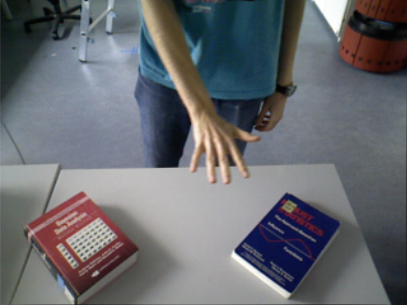
\includegraphics[width=0.32\linewidth]{w_scene.png}}
    \subfloat[\label{w_residuals}]{
        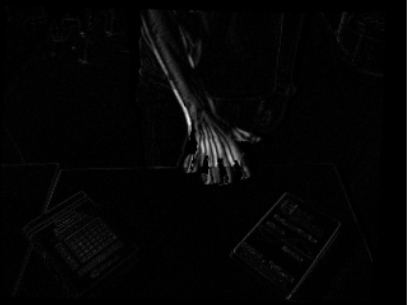
\includegraphics[width=0.32\linewidth]{w_residuals.png}}
    \subfloat[\label{w_weights}]{
        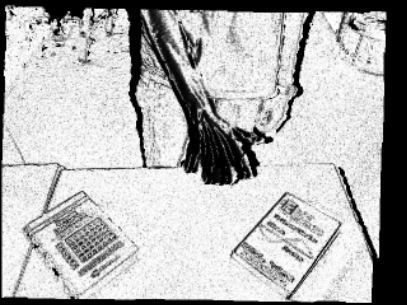
\includegraphics[width=0.32\linewidth]{w_weights.png}}
    \caption{Example of residual weighting: (a) a scene with a hand (outlier pixels) moving through; (b) the residuals calculated from \eqref{residual}, outlier pixels have much larger residuals than other pixels; (c) the weights of the pixels, which greatly reduced the influence of the outlier pixels. \cite{kerl2013robust}}
    \label{img_weighting}
\end{figure}

The Tukey function proposed in \cite{tukey1975mathematics} is among the earliest error-weighting functions used for robust estimation \cite{tykkala11direct}. It is computed using the median absolute deviation of the dataset, and is defined as follows:

\begin{equation}
\omega_{\text{Tukey}}(x)=\left\{
\begin{array}{ll}
{\left(1-\frac{x^{2}}{b^{2}}\right)^{2}} & {|x| \leq b} \\
{0} & {\text {else}}
\end{array}
\right.
\label{tukey}
\end{equation}

\noindent and for each residual the weight function is computed as:

\begin{equation}
w_{i}=\omega_{\text {Tukey}}\left(\frac{r_{i}}{\sigma_{\mathrm{r}}}\right)
\end{equation}

\noindent where $\sigma_r$ is the median absolute deviation of $\mathrm{r}$, and the parameter $b$ should be selected in accordance with the underlying outlier-free distribution of the data (e.g. $b=4.6851$ for 95\% asymptotic efficiency on standard normal distribution \cite{zhang1997parameter}). The Tukey function proves to be highly robust w.r.t both global and local robustness criteria \cite{chen2002influence}.

Apart from \eqref{tukey}, the Huber function proposed in \cite{huber2004robust} has also been widely used for robustification of noisy dataset. It suppresses the influence of large residuals by adjusting their terms to linear instead of quadratic:

\begin{equation}
\omega_{\text{Huber}}(x)=\left\{
\begin{array}{ll}
{1} & {|x| \leq k} \\
{\frac{k}{|x|}} & {\text{else}}
\end{array}
\right.
\label{huber}
\end{equation}

\noindent where the parameter $k$ should again be selected according to the underlying distribution of the data (e.g. $k = 1.345$ for 95\% asymptotic efficiency on standard normal distribution \cite{zhang1997parameter}). The effectiveness of Huber function in suppressing very large residuals is worse than Tukey function, but one advantage of Huber function is its convexity, which keeps the local minima of the original function without bringing about new interference for optimization.

Despite the theoretical effect of the two robust error functions, it is stated in the paper that the performance is not satisfying enough in the preliminary experiments. So an explicit modeling of the underlying distribution of the residuals is carried out to further enhance the robustness of the algorithm.

The distribution of all frame pairs are investigated on several datasets from the TUM-Dataset \cite{sturm12iros}. The accumulated histograms of the residuals of all successive frame pairs for some datasets are shown in Fig. \ref{histo}. As can be seen from the histograms and Fig. \ref{distribs}, a normal distribution or one with robust error function can not properly reflect the underlying distribution of residuals, leading to inappropriate weighting functions. On the other hand, a t-distribution \cite{lange1989robust} fits the observed histograms nicely, as can be seen in Fig. \ref{distribs}.

\begin{figure}[h]
    \centering
    \subfloat[\label{d_fr1desk}fr1/desk]{
        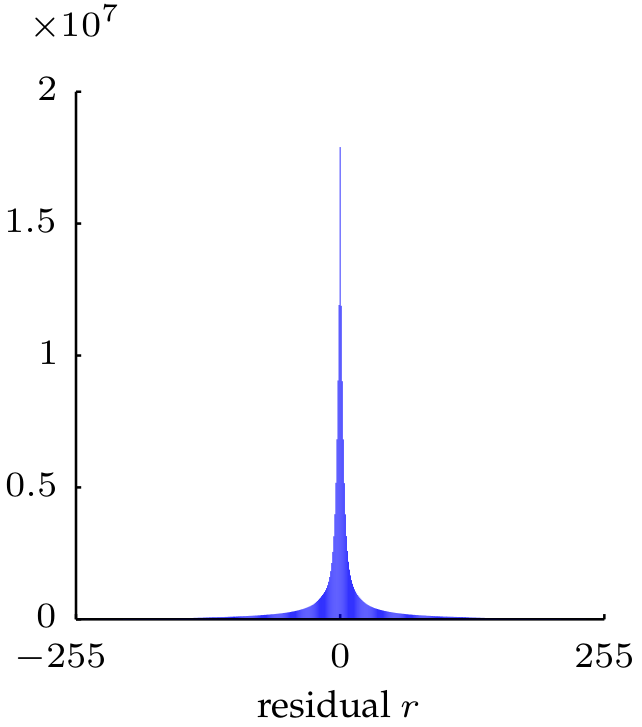
\includegraphics[width=0.32\linewidth]{fr1_desk.png}}
    \subfloat[\label{d_fr3sitting}fr3/sitting\_halfsphere]{
        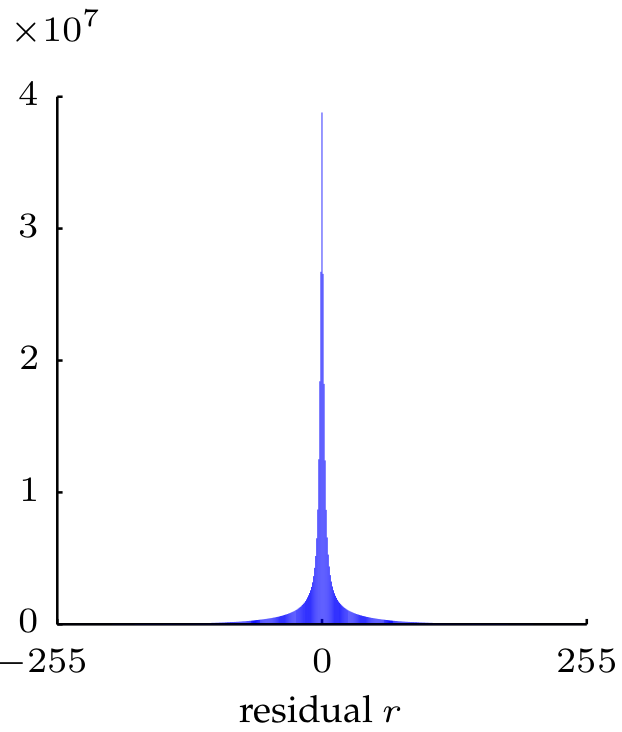
\includegraphics[width=0.32\linewidth]{fr3_sitting.png}}
    \subfloat[\label{d_fr3walking}fr3/walking\_halfsphere]{
        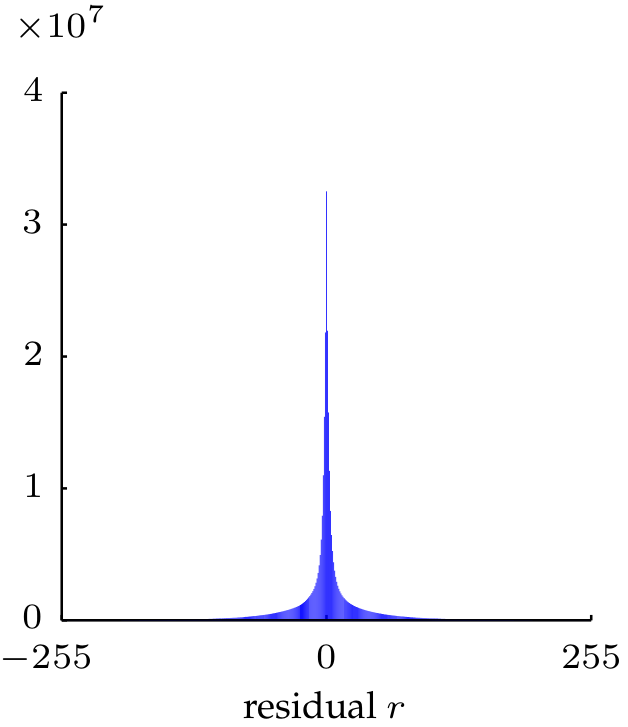
\includegraphics[width=0.32\linewidth]{fr3_walking.png}}
    \caption{Accumulated histogram of the residuals of all successive frame pairs from different datasets \cite{kerl2012odometry} (a) fr1/desk (b) fr3/sitting\_halfsphere (c) fr3/walking\_halfsphere}
    \label{histo}
\end{figure}

\begin{figure}[h]
    \centering
    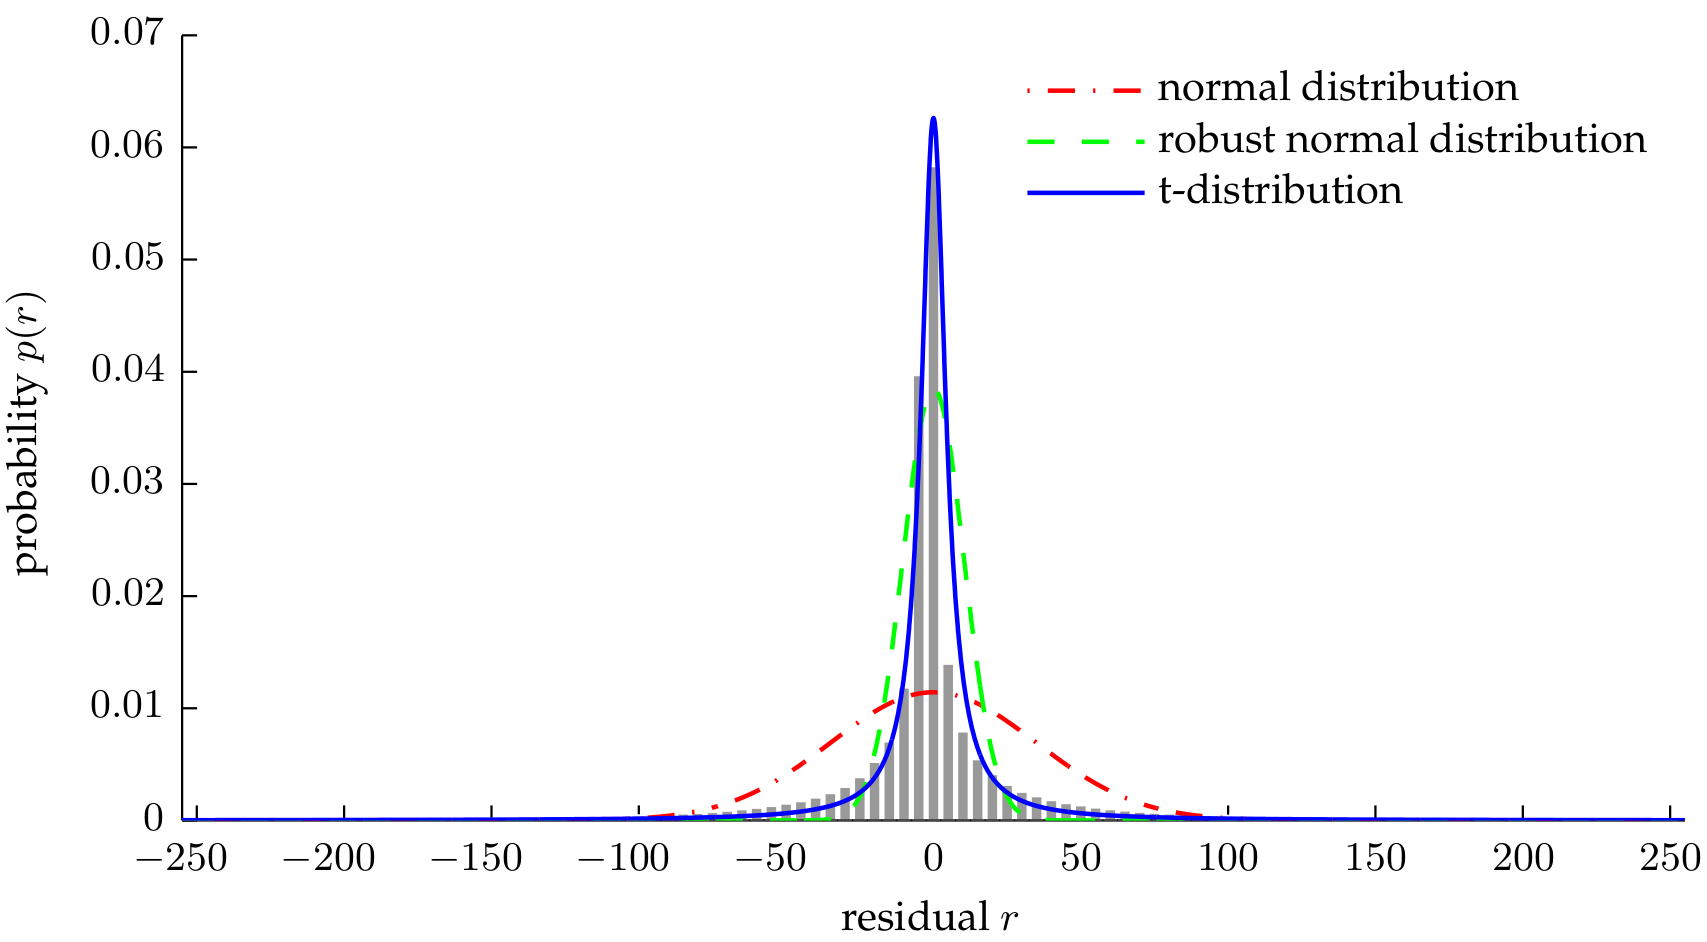
\includegraphics[width=\linewidth]{distribs.png}
    \caption{Modeling the distribution of residuals with various kind of models. \cite{kerl2012odometry}}
    \label{distribs}
\end{figure}

A t-distribution is defined as:

\begin{equation}
p(x | \mu, \sigma, \nu)=\frac{\Gamma\left(\frac{v+1}{2}\right)}{\Gamma\left(\frac{\nu}{2}\right) \sqrt{\pi \nu \sigma^{2}}}\left(1+\frac{1}{\nu} \frac{(x-\mu)^{2}}{\sigma^{2}}\right)^{-\frac{v+1}{2}}
\label{tdistrib}
\end{equation}

\noindent where $\mu$ is the mean, $\sigma^2$ the variance, $\nu$ the degree of freedom of the data and $\Gamma(x) = (x-1)!$ the gamma function. A t-distribution can be interpreted as a Gauss Mixture Model with infinite many centroids \cite{bishop2006pattern}, which is more flexible compared to the i.i.d. assumption in section 2.2. Each residual is weighted with its inverse variance considering \eqref{deriv} and \eqref{rwls}, and large residuals (outliers) are generated by centroids with high variances. These residuals will accordingly get low weights and thus suppressed.

The weight function $\omega(r_i)$ can be calculated from \eqref{deriv} and \eqref{tdistrib} as:

\begin{equation}
\omega_{\mathrm{t}}(r_i)=\frac{\nu+1}{\nu+\left(\frac{r_i}{\sigma_{\mathrm{t}}}\right)^{2}}
\label{weight_t}
\end{equation}

\noindent where the mean is set as $\mu = 0$ and the variance $\sigma_{\mathrm{t}}^2$ has to be iteratively solved using maximum likelihood estimation based on the current residuals:

\begin{equation}
\sigma_{\mathrm{t}, k+1}^{2}=\frac{1}{n} \sum_{i}^{n} \frac{\nu+1}{\nu+r_{i}^{2} / \sigma_{\mathrm{t}, k}^{2}} r_{i}^{2}
\end{equation}

\noindent which will converge in few iterations.

An example is shown in Fig. \ref{w_weights}, illustrating the weights of the residuals computed from the t-distribution. As can be discovered in the figure, the large residuals caused by the moving hand are weighted extremely low, which corresponds to an outlier-suppression behavior.

\subsection{Optimization Methods}

Conventionally, a (weighted) least square optimization problem can be solved by many standard methods such as gradient descent, Newton method, Gauss-Newton method, Levenberg-Marquardt method etc. Considering the convergence rate and the computational complexity, only Gauss-Newton method and Levenberg-Marquardt method will be discussed in this report.

The warping function \eqref{warpfunc} implies that the residual is not linear w.r.t camera motion $\boldsymbol{\xi}$, making \eqref{rwls} a non-linear optimization problem. Thus, a local linearization around $\boldsymbol{\xi} = \mathbf{0}$ using Taylor expansion is fisrt applied to enable the use of standard methods:

\begin{equation}
\begin{aligned}
r_{\text {lin}}\left(\boldsymbol{\xi}, \mathbf{x}_{i}\right) &=r\left(\mathbf{0}, \mathbf{x}_{i}\right)+\left.\frac{\partial r\left(\tau\left(\boldsymbol{\xi}, \mathbf{x}_{i}\right)\right)}{\partial \boldsymbol{\xi}}\right|_{\boldsymbol{\xi}=\mathbf{0}} \Delta \boldsymbol{\xi} \\
&=r\left(\mathbf{0}, \mathbf{x}_{i}\right)+J_{i} \Delta \boldsymbol{\xi}
\end{aligned}
\label{linear}
\end{equation}

\noindent where $J_i \in \mathbb{R}^{1 \times 6}$ is the Jacobian of the i-th pixel w.r.t. the 6-DOF camera motion in twist coordinate evaluated at $\boldsymbol{\xi} = \mathbf{0}$. Combining \eqref{residual} and \eqref{warpfunc} and applying the chain rule, the Jacobian can be calculated as:

\begin{equation}
\begin{aligned}
J_i = \left.\frac{\partial r\left(\tau\left(\boldsymbol{\xi}, \mathbf{x}_{i}\right)\right)}{\partial \boldsymbol{\xi}}\right|_{\boldsymbol{\xi}=\mathbf{0}}
=&\left.\frac{\partial I_{2}(\mathbf{y})}{\partial \mathbf{y}}\right|_{\mathbf{y}=\pi\left(\mathbf{p}\right)} \cdot
\left.\frac{\partial \pi(\mathbf{p})}{\partial \mathbf{p}}\right|_{\mathbf{p}=T\left(g(\mathbf{0}), \pi^{-1}\left(\mathbf{x}_{i}, Z_{1}\left(\mathbf{x}_{i}\right)\right)\right)} \\
\cdot &\left.\frac{\partial T\left(g(\boldsymbol{\xi}), \pi^{-1}\left(\mathbf{x}_{i}, Z_{1}\left(\mathbf{x}_{i}\right)\right)\right)}{\partial \boldsymbol{\xi}}\right|_{\boldsymbol{\xi}=\mathbf{0}}
\end{aligned}
\label{jacob_pre}
\end{equation}

\noindent which further yields

\begin{equation}
J_i=\left(\nabla I_{2, x} \quad \nabla I_{2, y}\right)\left(
\begin{array}{cccccc}
{f_{x} \frac{1}{z}} & {0} & {-f_{x} \frac{x}{z^{2}}} & {-f_{x} \frac{x \cdot y}{z^{2}}} & {f_{x}\left(1+\frac{x^{2}}{z^{2}}\right)} & {-f_{x} \frac{y}{z}} \\
{0} & {f_{y} \frac{1}{z}} & {-f_{y} \frac{y}{z^{2}}} & {-f_{y}\left(1+\frac{y^{2}}{z^{2}}\right)} & {f_{y} \frac{x \cdot y}{z^{2}}} & {f_{y} \frac{x}{z}}
\end{array}\right)
\label{jacob_res}
\end{equation}

Note that \eqref{jacob_pre} and \eqref{jacob_res} are only valid for pinhole camera model due to the projection and unprojection function $\pi$ and $\pi^{-1}$ used for computing derivatives.

As can be observed in \eqref{rwls} and \eqref{rwls_mp}, the weights only affect the scales of the corresponding residuals, and therefore can be incorporated into a diagonal matrix $W$ with $w_{ii} = \omega(r_i)$. Plugging \eqref{linear} into \eqref{deriv} and formulating in matrix notation yield:

\begin{equation}
J^{\top} W J \Delta \boldsymbol{\xi}=-J^{\top} W \mathbf{r}(\mathbf{0})
\label{gn_equation}
\end{equation}

\noindent where $J \in \mathbb{R}^{n \times 6}$ is the stacked matrix of all $J_i$. In the $k$-th iteration, an increment $\Delta \boldsymbol{\xi}$ is solved and integrated into the current camera motion with $\boldsymbol{\xi}_{k+1} = \log \left(\exp (\Delta\boldsymbol{\xi}) \cdot \exp (\boldsymbol{\xi}_{k})\right)$.

Similarly, the equation for motion increment using Levenberg-Marquardt method can be derived:

\begin{equation}
\left(J^{\top} W J+\lambda \operatorname{diag}\left(J^{\top} W J\right)\right) \Delta \boldsymbol{\xi}=-J^{\top} W \mathbf{r}(\mathbf{0})
\end{equation}

When the motion prior described in \eqref{rwls_mp} is also taken into account, \eqref{gn_equation} becomes:

\begin{equation}
\left(J^{\top} W J+\Sigma^{-1}\right) \Delta \boldsymbol{\xi}=-J^{\top} W \mathbf{r}(0)+\Sigma^{-1}\left(\boldsymbol{\xi}_{0}-\boldsymbol{\xi}_{k}\right)
\end{equation}

\noindent where the mean $\boldsymbol{\xi}_0$ can be set as the camera motion calculated from the last pair of frames by assuming the smoothness of motion, and the covariance matrix $\Sigma_{\text{prior}}$ need to be tuned.

\subsection{Image Pyramid}

The equations of estimating the camera motion iteratively given in the previous section are actually not valid when the camera motion is rather large, because the linearization is carried out around $\boldsymbol{\xi} = \mathbf{0}$. Therefore, a coarse-to-fine scheme is adopted to support the estimation of large $\boldsymbol{\xi}$: an image pyramid is built with image resolutions being halved at each layer (Fig. \ref{pyramid}). The motion estimation is first executed on the top layer with lowest resolution, and the estimation is iteratively propagated downwards, serving as initialization for the next layer. In this way, even large camera motions can be properly estimated.

\begin{figure}[h]
    \centering
    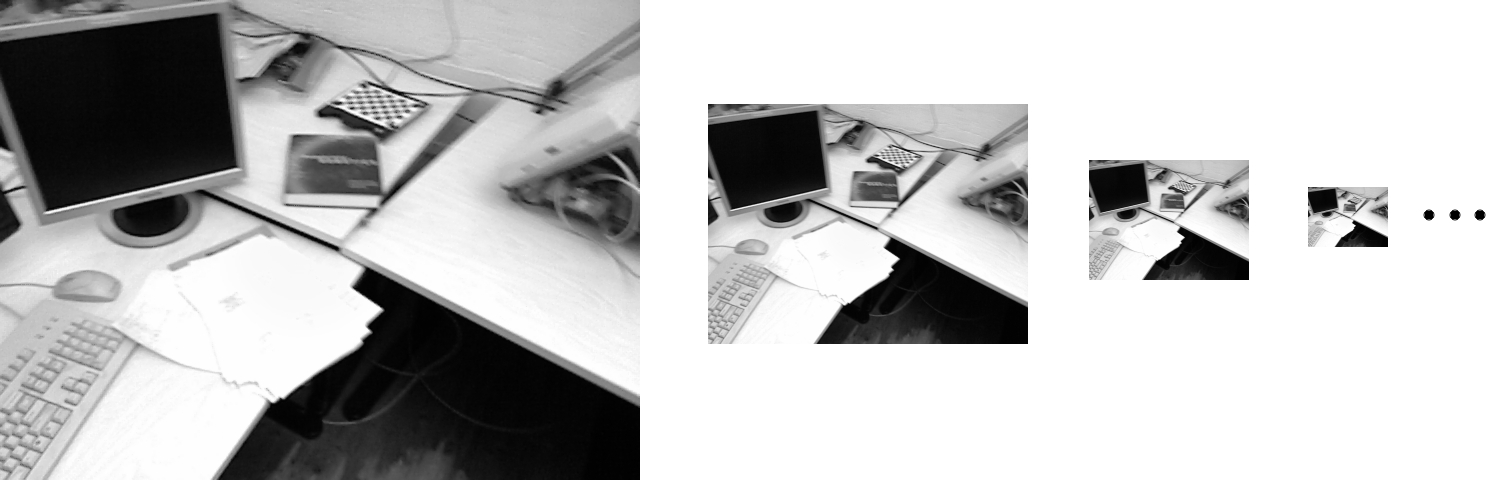
\includegraphics[width=\textwidth]{pyramid.jpg}
    \caption{Image pyramid built to enable larger camera motion with valid linearization. In each layer, the image resolution is halved and the corresponding intrinsic parameters are modified.}
    \label{pyramid}
\end{figure}

While halving the image resolution, the corresponding intrinsic parameters should also be properly adapted. This can be achieved by comparing the pixel coordinates between two neighboring layers $k$ and $k+1$:

\begin{equation}
2 \mathbf{x}^{(k+1)}+\frac{1}{2}=\mathbf{x}^{(k)}
\end{equation}

plugging into the projection equation $\mathbf{x}=\frac{1}{Z} K \mathbf{X}$ yields:

\begin{equation}
f_{x}^{(l+1)}=\frac{1}{2} f_{x}^{(l)}, \quad f_{y}^{(l+1)}=\frac{1}{2} f_{y}^{(l)}, \quad c_{x}^{(l+1)}=\frac{1}{2} c_{x}^{(l)}-\frac{1}{4}, \quad c_{y}^{(l+1)}=\frac{1}{2} c_{y}^{(l)}-\frac{1}{4}
\end{equation}

Note that the $(0, 0)$ coordinate is define at the center of the top-left pixel.

\section{Implementation}
The implementation of the described algorithm can be inspected in the gitlab repository \verb|RGBD_DVO| under \url{https://gitlab.vision.in.tum.de/s0010/rgbd_dvo} and mainly contains two classes:

\begin{itemize}
    \item The \verb|DirectOdometry| class implements the scheme of the algorithm discussed in section 2. The complete workflow is described in the pseudo-code \ref{algo_dvo}:
    \begin{algorithm}[h]
        \caption {Direct Visual Odometry}
        \label{algo_dvo}
        \begin{algorithmic}[1]
        \REQUIRE RGB-D frame stream
        \ENSURE Camera motion of all successive frame pairs
        
        \FOR{all succesive frame pairs}
            \FOR{layer in image pyramid (top-down)}
                \WHILE{not converged}
                    \STATE Compute residual image $\mathrm{r}(\boldsymbol{\xi}_k)$
                    \STATE Compute weight matrix $W$ from \eqref{weight_t}
                    \STATE Compute Jacobians $J$ from \eqref{jacob_res}
                    \STATE Compute motion increment $\Delta \boldsymbol{\xi}$ from \eqref{gn_equation}
                    \STATE Update camera motion $\boldsymbol{\xi}_{k+1} = \log \left(\exp (\Delta\boldsymbol{\xi}) \cdot \exp (\boldsymbol{\xi}_{k})\right)$
                \ENDWHILE
            \ENDFOR
        \ENDFOR
        \end{algorithmic}
    \end{algorithm}
    \item The \verb|Frame| class provides support for image frames and pyramids, including the storage of a image frame (RGB image and depth image) and the construction of image pyramid discussed in section 2.5. As frame pairs are taken successively, the image pyramid is calculated only once for each frame.
\end{itemize}

For the optimization step, both methods discussed in section 2.4 are implemented in the \verb|DirectOdometry| class, and the Gauss-Newton method is used for testing, as it requires no fine-tuning of hyper parameter (comparing to the $\lambda$ parameter in Levenberg-Marquardt method).

The user interface shows both the current RGB image and the final residual image of the current frame pair. The trajectory generated from odometry and the ground-truth are shown in different color in real time below the images (Fig. \ref{result}). After the whole process finishes, an alignment between the true and the estimated trajectories is executed to reduce the influence of possible local errors on the global trajectory.

\section{Performance measure and possible improvement}

The implementation of the algorithm described above is tested on the TUM-Dataset \cite{sturm12iros}. The absolute trajectory error (ATE) is used to measure the performance of odometry and to compare with the reference test results given in \cite{kerl2013robust}. The comparison of results are given in Table \ref{tab_results}.

\begin{figure}[h]
    \centering
    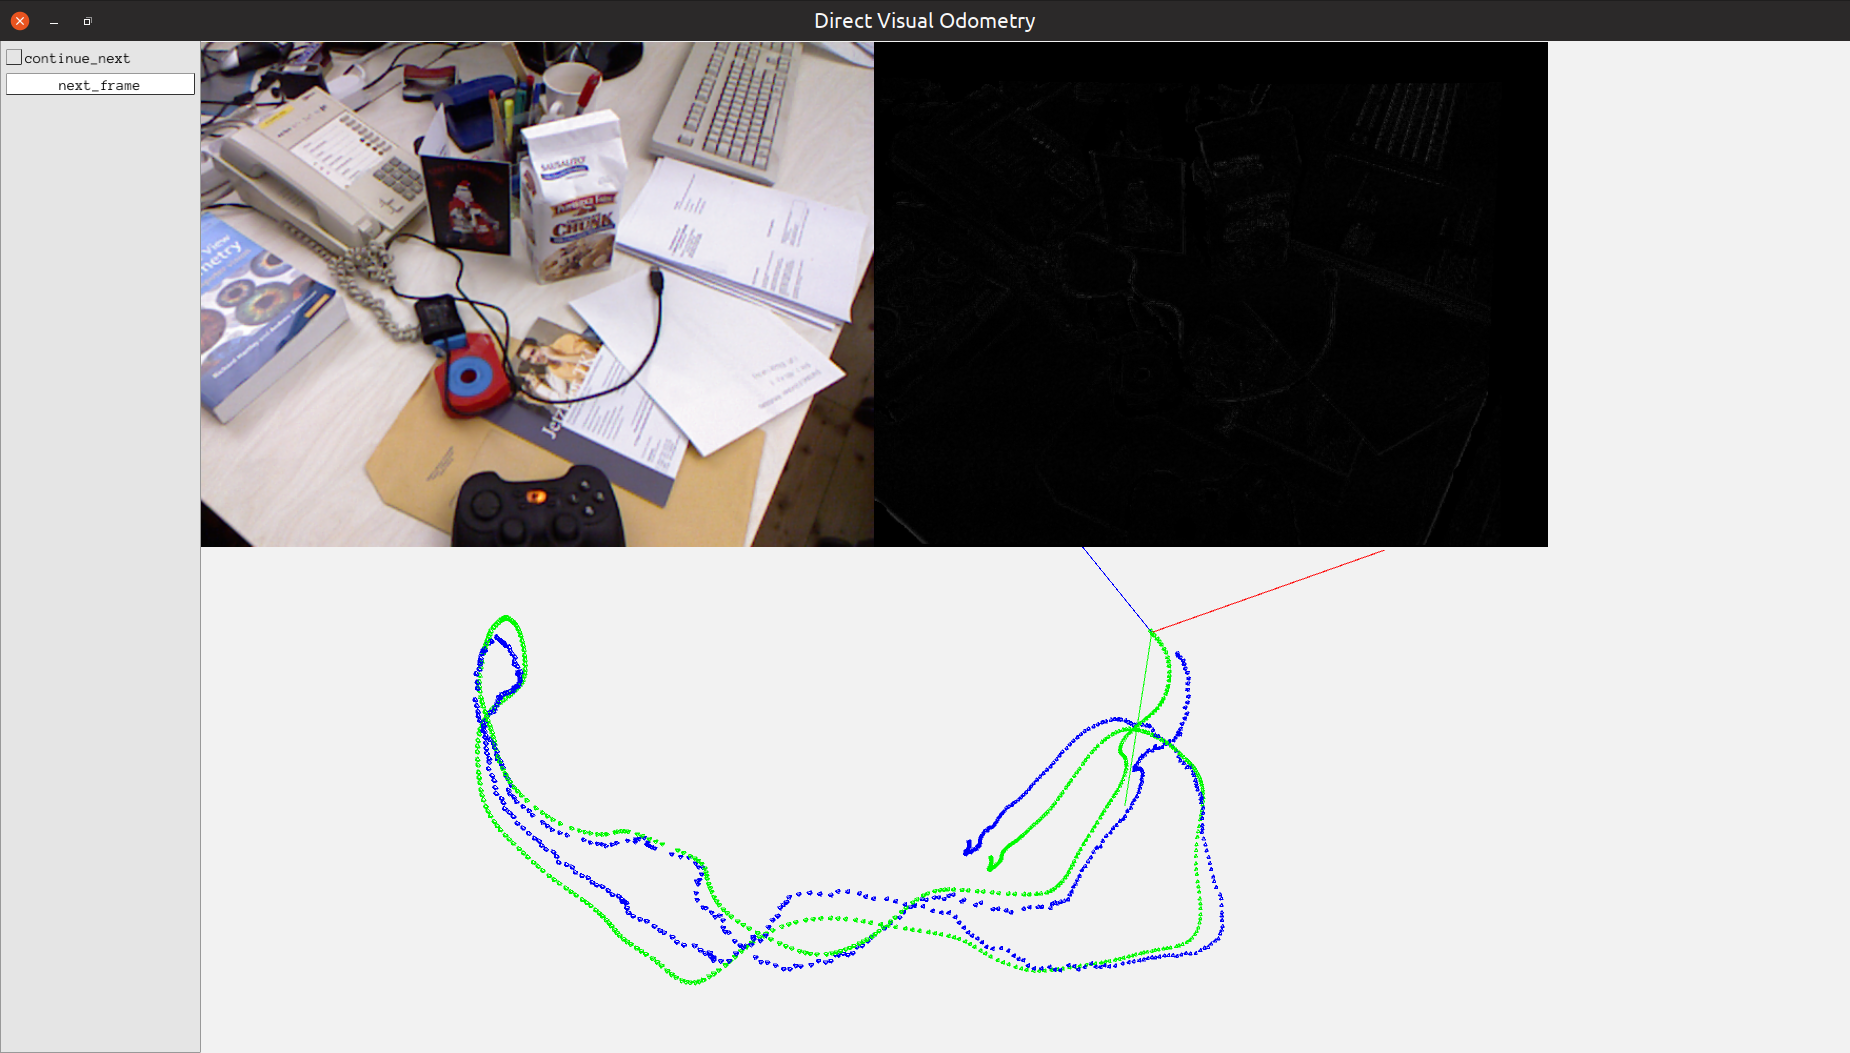
\includegraphics[width=\textwidth]{result.png}
    \caption{The user interface and one sample result of visual odometry from the manual implementation in the project running on the TUM-Dataset fr1/desk. The estimated trajectory is illustrated in blue, and the ground-truth in green.}
    \label{result}
\end{figure}

\begin{table}[h]
  \caption{Comparison of results from manual implementation and original paper}
  \label{tab_results}
  \begin{tabular}{ccl}
    \toprule
    Datasets & Manual implementation & Results given in \cite{kerl2013robust}\\
    \midrule
    fr1/desk & 0.0957 & 0.0687\\
    fr1/desk2 & 0.0725 & 0.0491\\
    fr2/desk & 0.0312 & 0.0188\\
    fr2/person & 0.0497 & 0.0345\\
  \bottomrule
\end{tabular}
\end{table}

As can be see from the table, the trajectory estimation given by the manual implementation is not as good as the results in the paper, but the difference also lies in an acceptable range. By fine-tuning some hyper parameters (depth of image pyramid, convergence condition of Gauss-Newton method etc.) and applying the following improvements, the performance can still be further enhanced:

\begin{itemize}
    \item Using Levenberg-Marquardt method instead of Gauss-Newton method. Although implemented in this project, Levenberg-Marquardt method is not used in the performance tests due to the parameter $\lambda$ that requires tuning. Levenberg-Marquardt method combines the advantages of gradient descent and Gauss-Newton method, and can usually yield faster convergence and better robustness \cite{madson2004methods}.
    \item Adjusting covariance matrix of motion prior. In the manual implementation, the covariance matrix of the motion prior is always set to identity, indicating that the motion prior is identical to the estimation from the last frame pair. Setting the covariance matrix to appropriate values can smoothen the generated trajectory and result in higher performance.
    \item Taking keyframes. The smoothness of the path can also be improved by using keyframing instead of simply estimating camera motion between neighboring frames. The camera motion will then be estimated between the current frame and its closest keyframe. The criteria of taking new keyframes should also be properly selected to avoid loss of image information during projection.
\end{itemize}

%%
%% The next two lines define the bibliography style to be used, and
%% the bibliography file.
\bibliographystyle{ACM-Reference-Format}
\bibliography{ref.bib}

\end{document}
\endinput
%%
%% End of file `sample-acmsmall.tex'.
